\subsubsection{Basic notions}\label{rnn_theory}

\acrfull{rnn}  is a type of network architecture that is applied to a multitude of problems, especially \acrshort{nlp} problems such as voice recognition or text translation, but it is also used for problems in which the data is arranged in time and has a certain relationship, such as in the case of stock market prediction or object detection in videos.
\newline


In summary, \acrshort{rnn} are networks are able to to work with sequential data models. An example using sequential data might be the following: A picture is shown with a circle drawn and you are asked in which direction the circle is going. Any answer to this question will be random and without any criteria. However, if several photos are shown and it is explained that they are photos taken before the first photo and in these photos, you can see that the circle follows a trajectory, then the answer to the question will be trivial because it is easy to predict where the circle will go.

\begin{figure}[H]
    \centering
    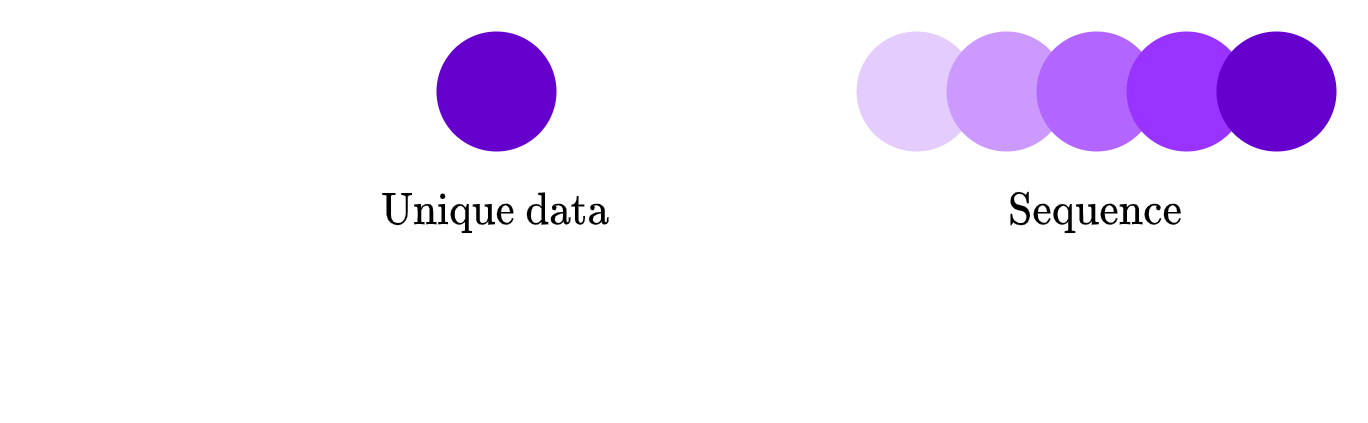
\includegraphics[width=10cm]{images/state-of-art/rnn/ball.png}
    \caption{Graphical example of a single piece of data vs. a sequence.}
    \label{fig:basic_network}
\end{figure}

In this way you can see the importance of having temporary information and how this can be used to solve predictions. Sequential information is present in the world in different forms: audio (bit sequence), text (sequence of characters or words) or values that change over time.
\newline

The way \acrshort{rnn} works is thanks to a concept known as sequential memory. Sequential memory is the ability to reproduce sequences of words, numbers, letters, symbols... of a human. For that reason, it is easy to say the alphabet and yet more difficult to say the alphabet backwards.
\newline

Using some kind of loop within the network, this sequential memory can be emulated so that a network architecture can use previous information to process the calculation of a new value. This information that is passed using the loop is known as the hidden state ($h$) and contains information from the previous input values.
\newline

When reference is made to an \acrshort{rnn}, we are talking about a network that at least one of the layers is recurrent and therefore has some kind of loop. That is, there can be an \acrshort{rnn} with only one recurrent layer or an \acrshort{rnn} with two recurrent layers or any kind of combination with at least one recurrent layer. Several examples are shown below:

\begin{figure}[H]
    \centering
    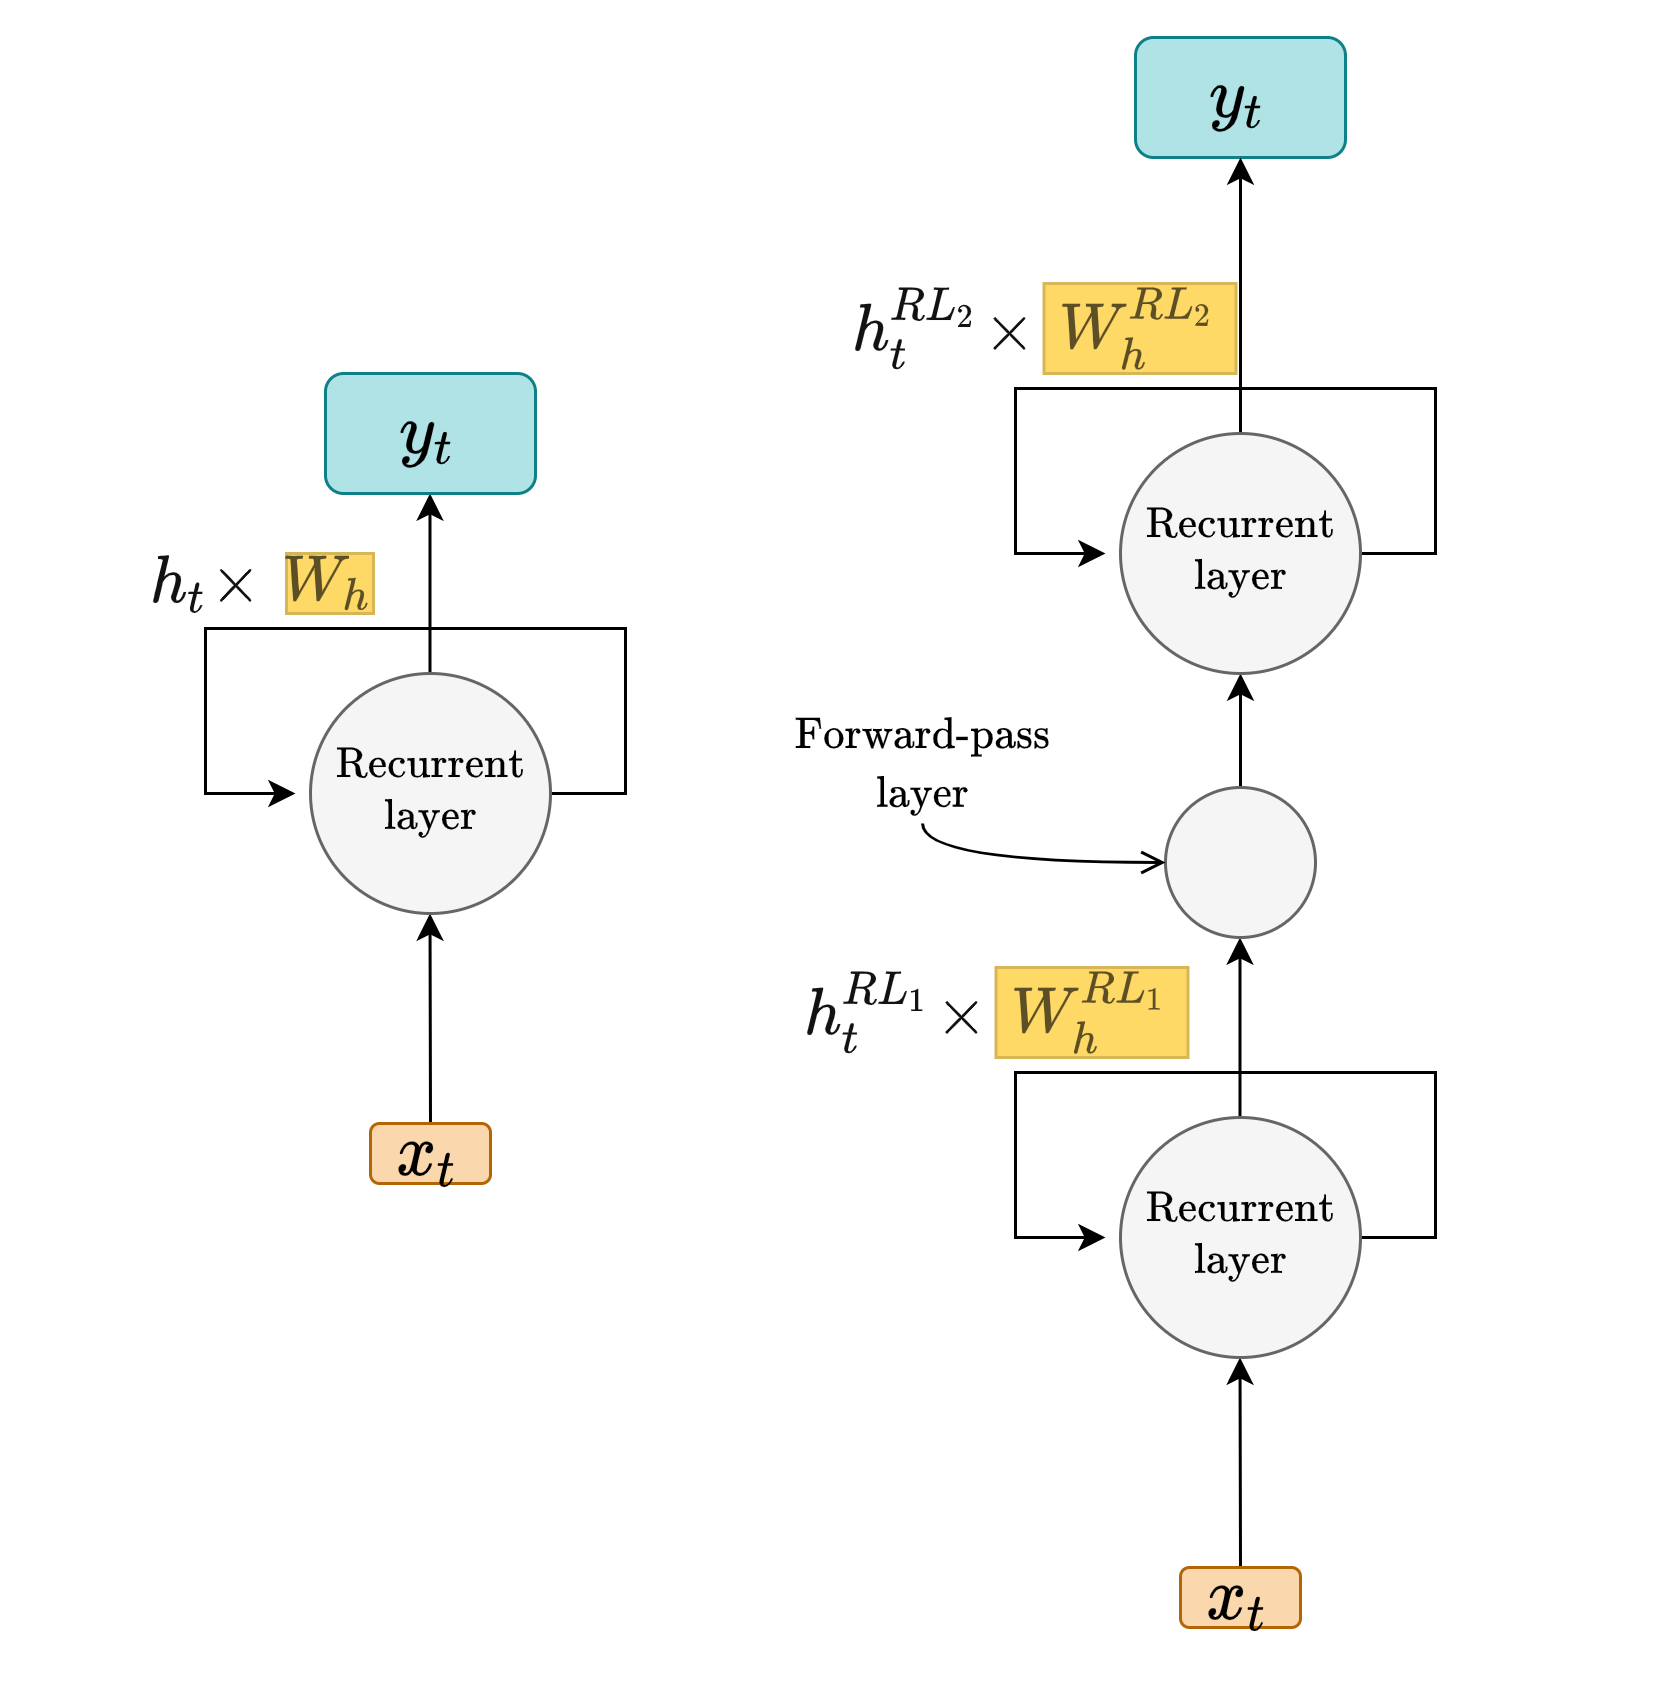
\includegraphics[width=10cm]{images/state-of-art/rnn/rnn-compact.png}
    \caption{Several examples of \acrshort{rnn}}
    \label{fig:rnn-compact}
\end{figure}

From now on, instead of representing the loop with a reflexive connection, it will be done using the horizontal axis for each of the iterations and in such a way that a linked network chain remains. This is the most common way to see the \acrshort{rnn} represented.
\newline

In the previous diagram, a new matrix has been introduced: $W_h$. This matrix is the proper weight matrix for vector h. Furthermore, as there can be several recurrent layers, to differentiate $W_h$ and $h$ the index $RL_i$ will be used, where $i$ is the number of the recurrent layer.
